\chapter{Задача о позиционировании случайного объекта за счет однократного изменения приращений его траектории} \label{chapt4}

\section{Введение}\label{sec:4.1}
%\setcounter{equation}{0}
В работе рассматривается одна из версий задачи позиционирования объекта, находящегося под воздействием случайных факторов. Цель состоит в том, чтобы минимизировать отклонение терминального положения объекта от заданного положения за счет однократного изменения величины приращений соответствующего случайного процесса в выбранный момент времени. При этом предполагается, что можно изменить интенсивность влияния случайных факторов, а также «направление» влияния. В качестве примера можно привести изменение положения паруса лодки, находящейся под воздействием случайного ветра. Другой пример - задача хеджирования европейского опциона в среднеквадратическом при условии, что портфель может быть изменен лишь один раз (отметим, что подобная задача при  $n$ - кратном изменении портфеля рассматривалась в работах [1], [2]).
В следующем разделе приводится постановка задачи и указывается, что она сводится к задаче оптимальной остановки. При этом требуется определить лишь оптимальное время изменения приращений процесса, а величина изменения определяется автоматически. В разделе \ref{sec:4.3} получены нижние оценки границы области продолжения в случаях, когда рассматриваемый процесс представляет собой броуновское движение со сносом и геометрическое броуновское движение. В разделе \ref{sec:4.4} приводятся результаты численных расчетов, которые сопоставляются с указанными оценками.

\section{Постановка задачи и ее сведение к задаче оптимальной остановки}\label{sec:4.2}

Считая, что у рассматриваемого объекта нет внутренних источников энергии, мы отождествляем воздействующий на него случайный процесс с самим объектом. Рассмотрим диффузионный процесс
$$dS_t=\mu(t,S_t) dt+\sigma(t,S_t) dW_t, \quad S_0=\mathrm {const},$$
где $W$ --- стандартный винеровский процесс. Будем считать, что положение объекта имеет вид
$$X_T = X_0+\gamma_0(S_\tau-S_0) +\gamma_\tau(S_T-S_\tau).$$
Здесь $X_0, \gamma_0$ --- начальные положение и интенсивность воздействия, а стратегия изменения интенсивности воздействия представлена парой  $(\gamma_\tau,\tau)$, где $\tau$  момент остановки относительно естественной фильтрации $\mathbb F=(\mathscr F_s)_{s\in [0,T]}$ винеровского процесса,  $\gamma_\tau $ --- $\mathscr F_\tau$ - измеримая случайная величина (в финансовой интерпретации $X$ --- капитал игрока, $\gamma$ --- его портфель, $S$ --- цена рискового актива).
Цель состоит в минимизации среднеквадратического отклонения положения объекта от заданного фиксированного уровня $H$  в терминальный момент времени $T$:
\begin{equation}
\label{eq:4.1.1}
\mathsf E[(X_T-H)^2] \to \min_{(\gamma_\tau,\tau)}.
\end{equation}

Данная задача сводится к задаче оптимальной остановки. Действительно, используя представление процесса $X_T$ и телескопическое свойство условного математического ожидания, находим:
\begin{align}
 \label{eq:4.1.2}
 & \mathsf E[(X_T-H)^2)]=\mathsf E[(X_0+\gamma_0 (S_\tau-S_0) +\gamma_\tau (S_T-S_\tau) - H)^2]= \nonumber \\
 & \mathsf E[\mathsf E((S_T-S_\tau)^2|\mathscr F_\tau)\gamma_\tau^2-2(\gamma_0(S_\tau-S_0) - \widehat H) \mathsf E((S_T-S_\tau) | \mathscr F_\tau)\gamma_\tau\nonumber \\
 &+(\gamma_0 S_\tau - \widehat H)^2],
\end{align}
где $\widehat H = H-X_0+\gamma_0 S_0$.  Если $\mathsf E((S_T-S_\tau)^2|\mathscr F_\tau) > 0$ , то функция (\ref{eq:4.1.2}) имеет единственный минимум по $\gamma_\tau$, который достигается в точке
\begin{equation}
 \label{eq:4.1.3}
 \gamma_\tau^*=(\widehat H-\gamma_0 S_\tau)\frac{\mathsf E((S_T-S_\tau) | \mathscr F_\tau)}{\mathsf E((S_T-S_\tau)^2|\mathscr F_\tau)}.
 \end{equation}
Подставляя (\ref{eq:4.1.3}) в (\ref{eq:4.1.2}), получаем задачу оптимальной остановки:
\begin{equation}
 \label{eq:4.1.4}
 \mathsf E\left[(\widehat H - \gamma_0 S_\tau)^2 \left( 1-\frac{\mathsf E((S_T-S_\tau) | \mathscr F_\tau)^2}{\mathsf E((S_T-S_\tau)^2 | \mathscr F_\tau)}\right)\right] \to \min_{\tau}.
 \end{equation}
Заметим, что если $\mathsf E((S_T-S_\tau)^2|\mathscr F_\tau) = 0$, то выражение (\ref{eq:4.1.4}) соответствует (\ref{eq:4.1.2}) с учетом обычного соглашения $0/0=0$.
Преобразуем выражение (\ref{eq:4.1.4}) для моделей броуновского движения со сносом и геометрического броуновского движения. В первом случае $dS_t=\mu dt+\sigma dW_t$,
\begin{align}
 \label{eq:4.1.5}
 &\mathsf E((S_T-S_\tau) | \mathscr F_\tau)=\mu(T-\tau),\nonumber \\
 &\mathsf E((S_T-S_\tau)^2 | \mathscr F_\tau)=(\mu(T-\tau))^2+\sigma^2(T-\tau).
 \end{align}		
Во втором $dS_t=\mu S_t dt+\sigma S_t dW_t$,
\begin{align}
 \label{eq:4.1.6}
 &\mathsf E((S_T-S_\tau) | \mathscr F_\tau)=S_\tau(e^{\mu(T-\tau)}-1),\nonumber \\
 &\mathsf E((S_T-S_\tau)^2 | \mathscr F_\tau)=S_\tau^2(e^{(2\mu+\sigma^2)(T-\tau)}-2e^{\mu(T-\tau)}+1).
 \end{align}				

Здесь $\mu\in\mathbb R$ и $\sigma>0$ --- некоторые константы. В обоих случаях задача (\ref{eq:4.1.4}) принимает вид
\begin{equation}
\label{eq:4.1.7}
\mathsf E[h(S_\tau)\phi(\tau)] \to \min_{\tau},
\end{equation}			

где $h(S_t)=(\widehat H - \gamma_0 S_t)^2$, а
\begin{equation}
 \label{eq:4.1.8}
 \phi(t)=\frac{\sigma^2}{\mu^2(T-t)+\sigma^2}
 \end{equation}
для модели броуновского движения со сносом, и
\begin{equation}
 \label{eq:4.1.9}
 \phi(t)=\frac{e^{2\mu(T-t)}(e^{\sigma^2(T-t)}-1)}{e^{(2\mu+\sigma^2)(T-t)}-2e^{\mu(T-t)}+1}
\end{equation}			

для модели геометрического броуновского движения. Заметим, что функция (\ref{eq:4.1.9}) имеет устранимую особенность в точке $T$.

\section{Оценка границы области остановки}\label{sec:4.3}

Для оценки областей остановки перейдем к интегральной форме задачи (\ref{eq:4.1.7}). Для этого, применим к $h(S_\tau)\phi(\tau)$ интегральную формулу Ито в пределах от $0$ до $\tau$:
 \begin{align*}
 &h(S_\tau)\phi(\tau)= h(S_0)\phi(0)+\int_0^t h(S_t)\phi'(t)dt +\int_0^t h'(S_t)\phi(t)dS_t\\
 &+\frac{1}{2}\int_0^t h''(S_t)\phi(t)\sigma^2(S_t)dt=h(S_0)\phi(0)+\int_0^t h(S_t)\phi'(t)\\
 &+h'(S_t)\phi(t)\mu(S_t)+\frac{1}{2}h''(S_t)\phi(t)\sigma^2(S_t)dt+\int_0^t h'(S_t)\phi(t)\sigma(S_t)dW_t
 \end{align*}
Заметим, что $\mathsf E\int_0^T (h'(S_t))^2\sigma^2(S_t)\phi^2(t)dt<\infty,$ так как $(h'(S_t))^2\sigma^2(S_t)$ является полиномом не более чем четвертой степени от случайной величины $S_t$, и $\phi(t)$ --- непрерывная функция. Следовательно, процесс $M_t=\int_0^t h'(S_t)\sigma(S_t)\phi(t)dW_t$ является мартингалом, и $\mathsf E M_t=0$.
Таким образом, задача (\ref{eq:4.1.7}) принимает вид
\begin{equation}
 \label{eq:4.2.1}
h(S_0)\phi(0)+\mathsf E\left [\int_0^\tau F(t,S_t)dt \right ] \to \min_{\tau},
\end{equation}
где
\begin{equation}
 \label{eq:4.2.2}
F(t,s)=h(s)\phi'(t)+ h'(s)\phi(t)\mu(s)+\frac{1}{2}h''(s)\phi(t)\sigma^2(s).
\end{equation}
Пусть $\tau$  любой момент остановки. Положим
$$\tau^*=\inf_t\{t\ge 0: F(t,S_t) \ge 0\} \wedge T.$$

Тогда $\int^{\tau}_0 F(t,S_t)dt \ge \int^{\tau^*}_0 F(t,S_t)dt$  на множестве $\{\tau < \tau^*\}$, и справедливо неравенство
\begin{equation*}
 \label{eq:4.2.3}
\int^{\tau \vee \tau^*}_0 F(t,S_t)dt \le \int^{\tau}_0 F(t,S_t)dt.
\end{equation*}
Это позволяет сузить интервал поиска оптимального момента $\tau$ с $[0,T]$ до $[\tau^*,T]$.
Рассмотрим <<область продолжения>>  $\mathcal C=\{(t,s): F(t,s) \le 0\}$, определяющую момент остановки $\tau^*$. Сразу заметим, что если $\mu=0$, то $\tau^*=0$ так как $F(t,s) > 0$ для модели броуновского движения со сносом, и $F(t,s) > 0$ при $s>0$ для модели геометрического броуновского движения. Отметим также, что при этом $\gamma^*_\tau=0$ при любом $\tau$ в силу (\ref{eq:4.1.3}) и (\ref{eq:4.1.5}), (\ref{eq:4.1.6}). Далее рассматривается случай $\mu \neq 0$.
Для исследуемых моделей, функция $F(t,s)$ является квадратической: $F(t,s)=a(t)s^2+b(t)s+c(t)$. В случае броуновского движения со сносом имеем:
\begin{align*}
&a(t)=\gamma_0^2 \phi^\prime(t) > 0,\\
&b(t)=2\gamma_0^2\mu \phi(t)-2H\gamma_0 \phi^\prime(t),\\
&c(t)=(\gamma_0^2 \sigma^2-2H \gamma_0 \mu) \phi(t)+H^2 \phi^\prime(t).
\end{align*}
Вычислим дискриминант
\begin{align*}
D(t)= b^2(t)-4a(t)c(t)&=(2\gamma_0^2\mu \phi(t)-2H\gamma_0 \phi^\prime(t))^2\\
&-4 \gamma_0^2 \phi^\prime(t) [(\gamma_0^2 \sigma^2-2H \gamma_0 \mu) \phi(t)+H^2 \phi^\prime(t)]\\
&=4\gamma_0^4[\mu^2\phi^2(t)-\sigma^2\phi(t)\phi^\prime(t)].
\end{align*}

Заметив, что $\phi^2(t)=\frac{\sigma^2}{\mu^2}\phi^\prime(t)$, получаем
$$D=4\gamma_0^4\sigma^2 \phi^\prime(t) [1-\phi(t)] \ge 0.$$
Таким образом, уравнение $F(t,s)=0$ имеет два вещественных корня $s_1(t)<s_2(t)$, $t<T$; $s_1(T)=s_2(T)$, а область продолжения, определяющая момент $\tau^*$, имеет вид
$$\mathcal C=\{(t,s): F(t,s) \le 0\}=\{(t,s): s_1(t) \le s \le s_2(t)\}.$$

Функции $s_1(t), s_2(t)$ монотонны на всем интервале $[0,T]$.
Действительно,
\begin{align}
 \label{eq:4.2.4}
s_{1,2}(t)&=\frac{-b(t) \pm \sqrt D(t)}{2 a (t)}=\frac{\widehat H}{\gamma_0}-\frac{\mu \phi(t)}{\phi^\prime(t)} \pm \sigma\sqrt{
\frac{1-\phi(t)}{\phi^\prime(t)}}=\\
&=\frac{\widehat H}{\gamma_0}-\frac{\sigma^2}{\mu}-\mu(T-t) \pm \sqrt{\mu^2(T-t)^2+\sigma^2(T-t)}. \nonumber
\end{align}
Следовательно,
\begin{equation}
 \label{eq:4.2.5}
s_{1,2}^\prime(t)=\mu \mp \frac{1}{2} \frac{2 \mu^2 (T-t) + \sigma^2}{\sqrt{\mu^2(T-t)^2+\sigma^2(T-t)}};
\end{equation}
Из неравенства
\begin{equation*}
(\mu (T-t) + \frac{\sigma^2}{2\mu})^2=\mu^2 (T-t)^2 +\sigma^2 (T-t)+\frac{\sigma^4}{4\mu^2}>\mu^2(T-t)^2+\sigma^2(T-t)
\end{equation*}
вытекает, что $s_{1}^\prime(t)<0, s_{2}^\prime(t)>0$ при $\mu>0$ и $s_{1}^\prime(t)>0, s_{2}^\prime(t)<0$ при $\mu<0$.
Для геометрического броуновского движения со сносом:
\begin{align*}
&a(t)=\gamma_0^2((\sigma^2+2\mu)\phi(t)+\phi^\prime(t)),\\
&b(t)=-2\widehat H\gamma_0(\mu \phi(t)+\phi^\prime(t)),\quad c(t)=H^2 \phi^\prime(t),
\end{align*}
Рассмотрим дискриминант
\begin{equation*}
D(t)=b^2(t)-4a(t)c(t)=4 H^2 \gamma_0^2\phi(t) [\mu^2\phi(t)-\sigma^2 \phi^\prime(t)].
\end{equation*}
Границы области $\mathcal C$ имеют вид
\begin{equation}
 \label{eq:4.2.6}
s_{1,2}(t)=\frac{H}{\gamma_0}\frac{\mu\phi(t)+\phi^\prime(t)\pm \sqrt{\mu^2\phi^2(t)-\sigma^2\phi(t)\phi^\prime(t)}}{(\sigma^2+2\mu)\phi(t)+\phi^\prime(t)}.
\end{equation}
С использованием правила Лопиталя, после простых, но громоздких вычислений находим, что $D(T)=\lim_{t \to T} D(t)=0$. Таким образом, $s_{1}(T)=s_{2}(T)$. Численные эксперименты показывают, что, как и в случае броуновского движения со сносом, верхняя граница области $\mathcal C$ является графиком монотонно убывающей функции, а нижняя --- графиком монотонно возрастающей функции.

\section{Разностная схема}\label{sec:4.4}

Введем функцию Беллмана
\begin{equation}
\label{eq:4.3.1}
v(t,s)=\inf_{\tau \in \mathcal T_t} \mathsf E \left[ h(S^{t,s}_\tau)\phi(\tau) \right]
\end{equation}
где $\mathcal T_t$ множество моментов остановки, со значениями на интервале $[t,T]$, и $S^{t,s}$ удовлетворяет условию  $S^{t,s}_t=s$. Согласно общей теории оптимальной остановки $v$ является вязкостным решением уравнения Гамильтона-Якоби-Беллмана
\begin{equation}
\label{eq:4.3.2}
\min{\left\{v_t - [\mu(x)v_{s}+\frac{1}{2}\sigma^2(s) v_{ss}],h(s)\phi(t)-v\right\}}=0,\ \  (t,s)\in G,
\end{equation}
см., напр., [3, теорема 7.7].
Кроме того, очевидно, что $v$ удовлетворяет граничному условию:
\begin{equation}
 \label{eq:4.3.3}
v(T,s)=h(s)\phi(T).
\end{equation}
Используемые здесь и далее понятия теории вязкостных решений являются стандартными и изложены во многи источниках: см., в частности, [4], [5], [3].
Для модели броуновского движения со сносом, $G=[0,T] \times\mathbb R$, $\mu, \sigma$ являются константами.
В модели геометрического броуновского движения,$G=[0,T] \times [0,+\infty)$, $\mu(s)=\mu s, \sigma(s)=\sigma s$.
Исходя из (\ref{eq:4.3.1}), нетрудно показать, что функция $v$, как и $h$  имеет квадратичный рост: $v(t,s) \le c(1+s^2)$.

Напомним, что если для любых (полунепрерывного сверху) вязкостного субрешения $u$ и (полунепрерывного снизу) вязкостного суперрешения $v$, удовлетворяющих условию полиномиального роста,
и таких что $u(T,s) \le v(T,s)$, справедливо неравенство $u(t,s) \le v(t,s)$, $(t,s) \in G$, то говорят что имеет место теорема сравнения.
 Для задачи (\ref{eq:4.3.2}) (\ref{eq:4.3.3}) теорема сравнения может быть доказана с использованием методов [3, Теорема 7.8].

Как известно (см. [6]) наличие теоремы сравнения гарантирует сходимость разностной схемы, при условии что последняя обладает свойствами аппроксимации, монотонности и устойчивости. Не вдаваясь в подробности, отметим лишь что приводимая ниже схема (относяшаяся к известному классу схем [7]) обладает указанными свойствами. Проверка этого утверждения осуществляется стандартными средствами.

Рассмотрим прямоугольную сетку
\begin{align*}
\overline G_h=\{(ih_1,jh_2): 0\le i\le I, J_{\min}\le j\le J_{\max}\},\\
Ih_1=T, \quad h_2J_{\min}=S_{\min}, \quad h_2J_{\max}=S_{\max}.
\end{align*}
Здесь $I,J,i,j$ --- целые числа, $h=(h_1,h_2)$ --- шаг сетки. Узлы $$z_{ij}=(ih_1,jh_2), \quad 0 \le i<I, \quad J_{\min}<j<J_{\max}$$
назовем внутренними, а остальные узлы --- граничными. Множества внутренних и граничных узлов обозначим через $G_h$ и $\partial G_h$ соответственно. Каждому внутреннему узлу поставим в соответствие уравнение для сеточной функции $v_{ij}=v(z_{ij})$:
\begin{align*}
0&=\min \left\{\frac{v_{i+1,j}-v_{i,j}}{h_1}+\mu(s_{j})\frac{v_{i+1,j+1}-v_{i+1,j}}{h_2}\right.\\
&+\left.\frac{\sigma^2(s_{j})}{2}\frac{v_{i+1,j+1}-2v_{i+1,j}+v_{i+1,j-1}}{h_2^2},h(s_{j}) \phi(ih_1)-v_{i,j}\right\}.
\end{align*}
Здесь $s_{j}=jh_2$, а уравнение справедливо как для случая броуновского движения со сносом, так и для геометрического броуновского движения соответственно. Отметим, что выбранный способ аппроксимации первой производной по пространственной переменной обеспечивает монотонность данной (явной) схемы. В граничных узлах ставится условие Дирихле
\begin{equation}
 \label{eq:4.3.4}
v_{ij}=h(s_{j}) \phi(ih_1),\ \ z_{ij}=(ih_1,jh_2) \in \partial G_h.
\end{equation}

Перейдем к описанию численных экспериментов. Для модели броуновского движения со сносом задача решалась при следующих входных данных: $T=10$, $H=4$, $X_0=1$, $S_0=10$, $\gamma_0=2$, $\mu=0.1$, $\sigma=0.4$. Граница области остановки (пунктирная линия) и её нижняя оценка (сплошная линия) представлены на рис. \ref{fig:4.1}.
\begin{figure}[h!]
        \centering
          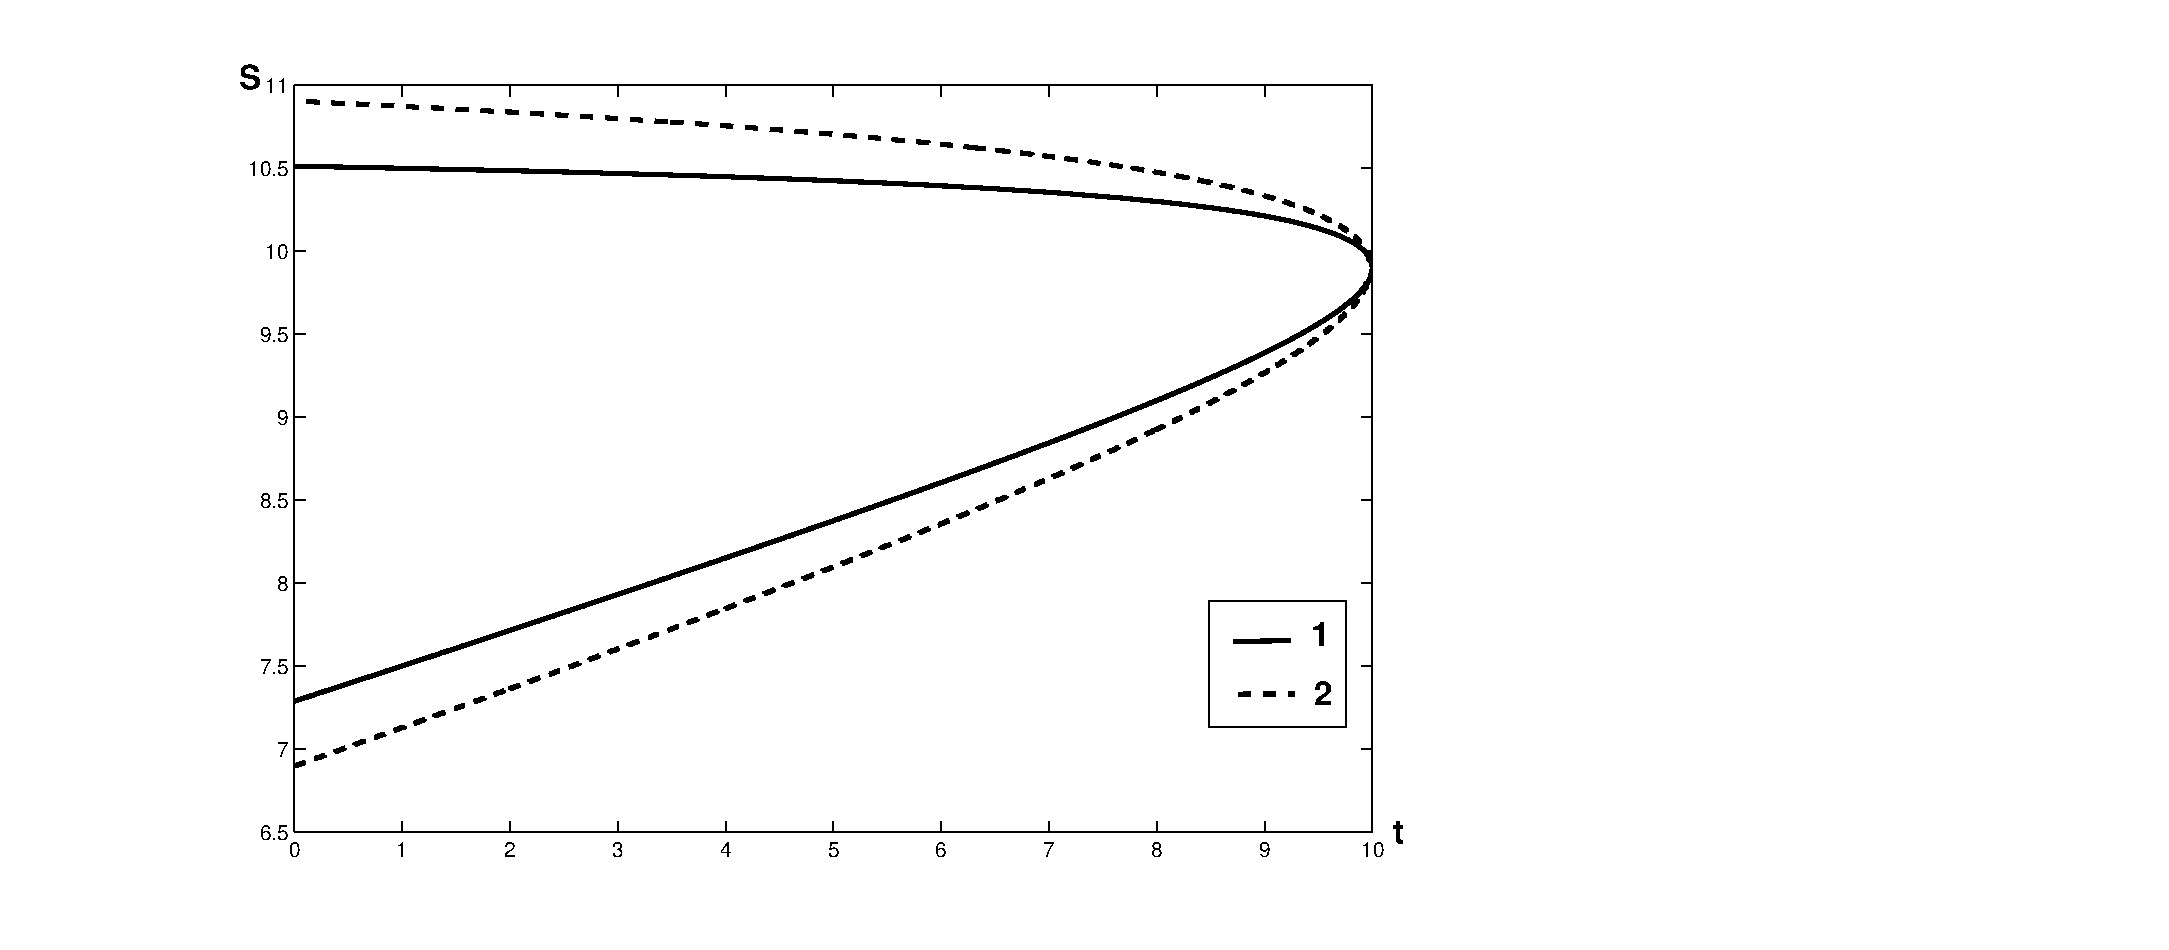
\includegraphics[width=1\textwidth]{graff_bash.eps}
         \caption{Граница области остановки и её нижняя оценка (\ref{eq:4.2.4}) для модели броуновского движения со сносом.}
          \label{fig:4.1}
\end{figure}

Можно отметить, что полученная в результате численных расчетов граница качественно ведет себя так же, как и её нижняя оценка. Величина погрешности зависит от параметров, но приведенная на рис. \ref{fig:4.1} картина является типичной. Отметим, что выражения
\begin{equation}
 \label{eq:3.5}
 s_{1,2}(0)-S_0=\frac{H-X_0}{\gamma_0}-\frac{\sigma^2}{\mu}-\mu T \pm \sqrt{\mu^2 T^2+\sigma^2 T}
\end{equation}
имеют при малых  $\mu \neq 0$ одинаковый знак, то есть $S_0$ не попадает в область продолжения $\mathcal C$. Данный вывод подтверждается численными расчетами.

Для модели геометрического броуновского движения картина несимметрична и, в типичном случае, верхняя граница области остановки оценивается менее точно чем нижняя. Соответствующие графики, для входных данных:$T=10$,$H=4$, $X_0=1$, $S_0=15$, $\gamma_0=0.2$, $\mu=0.1$, $\sigma=0.4$, представлены на \ref{fig:4.2}.

\begin{figure}[h!]
        \centering
          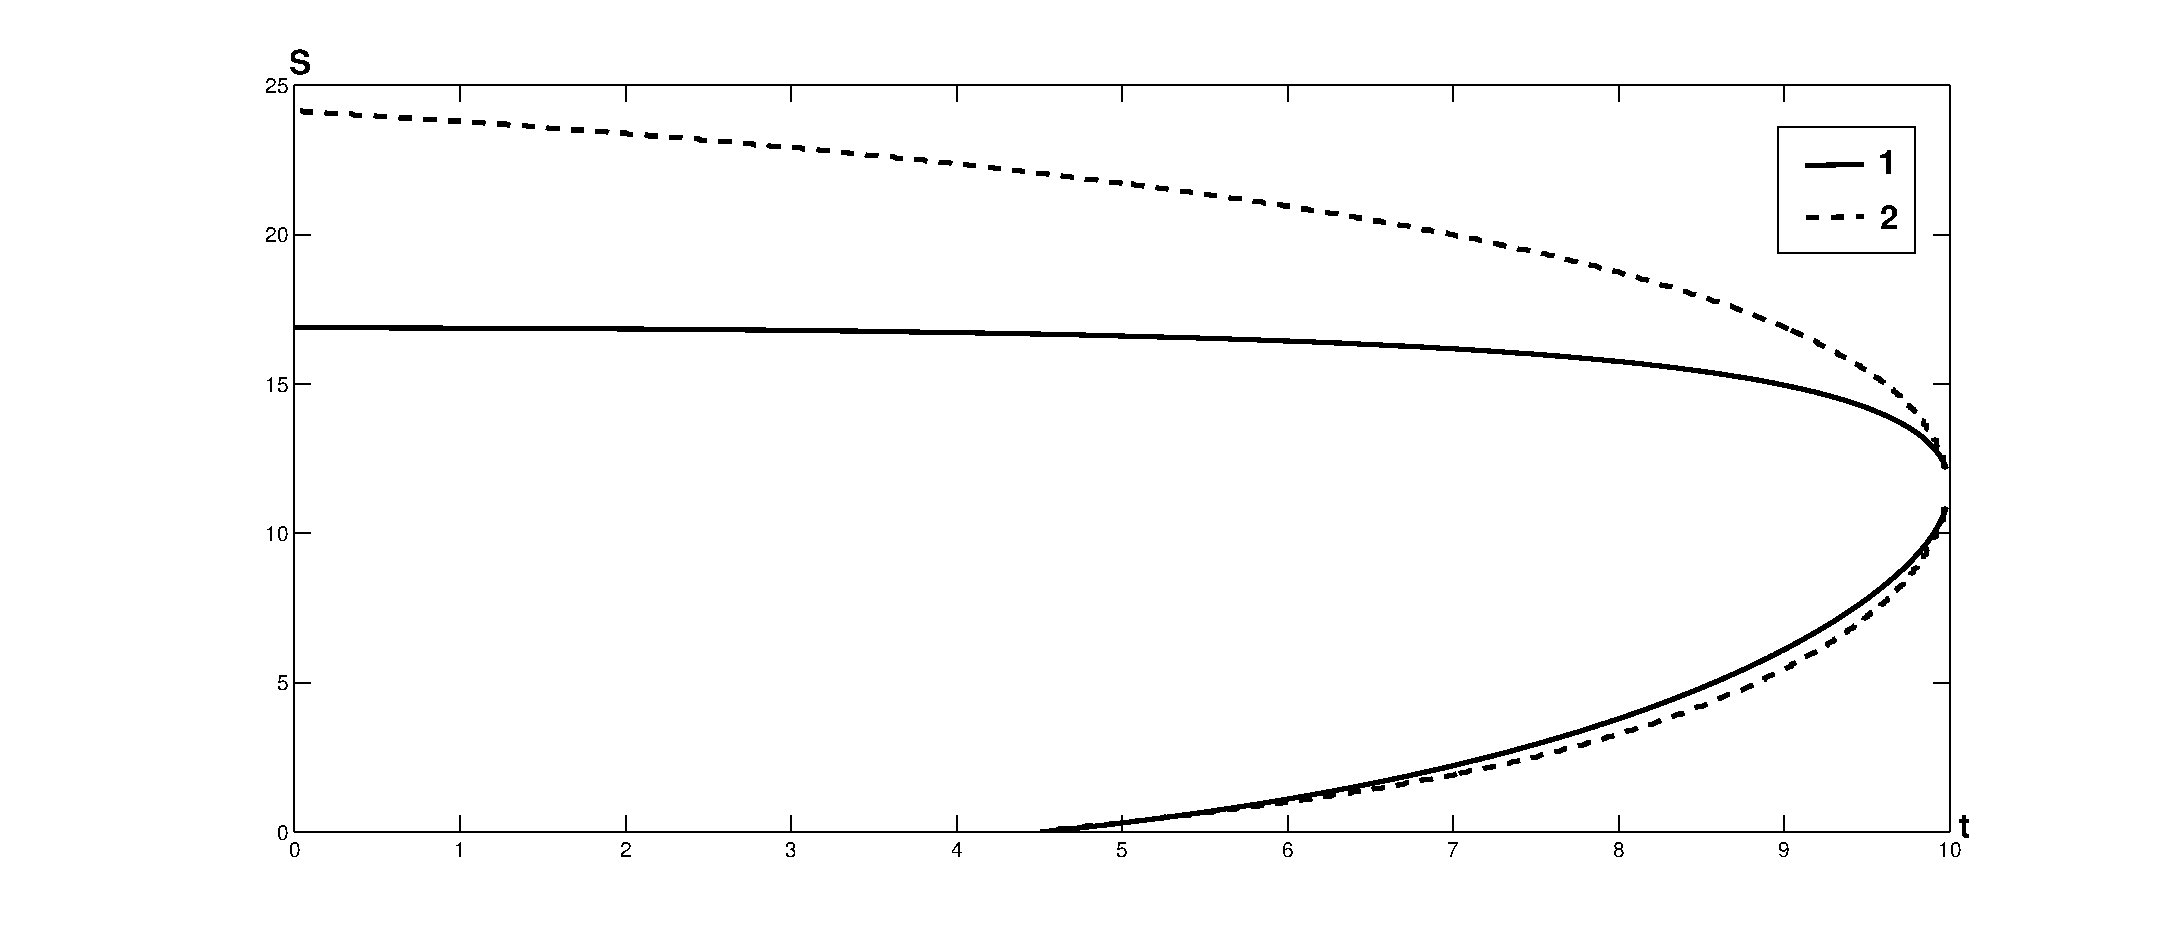
\includegraphics[width=1\textwidth]{graff_bs.eps}
          \caption{Граница области остановки и её нижняя оценка (\ref{eq:4.2.6}) для модели геометрического броуновского движения.}
          \label{fig:4.2}
\end{figure}

Отметим, что область остановки определяется лишь той частью границы, которая находится выше оси абсцисс.
Таким образом, проведенные эксперименты позволяют сделать вывод о том, что полученные в разделе \ref{sec:4.3} оценки дают удовлетворительное качественное описание оптимальных областей остановки.

\clearpage 